This section implements the Todo application using the BLoC package in order to handle the state. 
\subsubsection{Base funtionalities}  \label{par:todo_app_inherited_widget_introduction}

\paragraph{States - }
\label{subpar:todo_app_bloc_core_state}
The application state is decomposed in four smaller states: the state of the list, the state of the filtered list, the state of the statistics and the state of the tab. The state of the list contains the whole list of todos. The state of the filtered list contains a filter, of type VisibilityFilter, and a list of todos matching that filter value. The state of the stats contains an int number indicating the number of completed todos. Lastly, the state of the tab contains the value of the HomePage’s active tab. The state of the list and the state of the tab are independent. The state of the filtered list and the state of the stats,  instead, are directly linked to the state of the list. They will,  indeed, react to the changes in the state of the list and update consequently. 

\paragraph{The states of the list of todos - }
\label{subpar:todo_app_bloc_core_state}
First of all we start defining and naming the possible states of the list of todos. These states are only two: \textit{TodosLoadingState} and \textit{TodoLoadedState}. The \textit{TodosLoadingState} state indicates that the list of todos is still loading. The \textit{TodoLoadedState} state, instead, indicates that the list of todos has been successfully fetched from the database and is available. In order to define these two states, a new abstract class is created. It is called TodosState. It must extend the Equatable class. The  Equatable class is useful to define equality between states without the need to override the equality operator in every state class. The \textit{TodosLoadingState} does not contains any other information. The \textit{TodosLoadedState} contains, instead, a list filled with todos instances.
\begin{code}
\mbox{}\\
\captionof{listing}{Todo app – Bloc - states definition for the list of todos} \mbox{}
\label{code:2.14}
\begin{minted}[bgcolor=bluepoli!10]{dart}

abstract class TodosState extends Equatable{
  const TodosState();
  
  @override
  List<Object> get props => [];
}
class TodosLoadingState extends TodosState{

  @override
  String toString() => 'TodosState - TodosLoadingState';
}
class TodosLoadedState extends TodosState{
   final List<Todo> todos;
   const TodosLoadedState(this.todos);
   
   @override
   List<Object> get props => [todos];
   
   @override
   String toString() => 'TodosState - TodosLoadedState';
} 
\end{minted}
\mbox{}
\end{code}


\paragraph{The state of the filtered list and the filter - }
\label{subpar:todo_app_bloc_core_state}
Also in this case there are only two possible states: \textit{FilteredTodosLoadingState} and \textit{FilteredTodosLoadedState}. The \textit{FilteredTodosLoadingState} state identifies the fact that the filtered list hasn’t been computed (or todos fetched) yet. The  \textit{FilteredTodosLoadedState} state, instead,  identifies the fact that the list of todos has been successfully fetched and the filtered list computed. It contains two variables: a VisibilityFilter and a List of todos. An abstract class,  called \textit{FilteredTodosState}, must be created and extended with Equatable class. All the other state classes, belonging to the state relative to the filtered list, will extend the \textit{FilteredTodosState} abstract class. Someone can notice that,  the state of the filtered list, contains two different aspects of the application's state: the filter and the filtered list. In this case it is possible to further split the state creating two separated blocs, handling respectively the filter and the filtered list. From a general point of view, the state should be divided into as many pieces as possible to keep things clean and well separated,  like we do for classes and methods. However, the BLoC pattern does not specify how granular should the state fragmentation be and,  theoretically, we could decide to use a single bloc to handle the whole application ‘s state,  like in Redux. In this particular case,  I decided to implement a trade-off keeping the filter and the filtered list in the same bloc. They concern,  indeed, two similar aspects of the data. Splitting them,  would require the bloc of the filtered list to depend on the bloc of the filter also, raising its dependencies from one bloc to two blocs (the bloc of the todos and the bloc of the filter).
\begin{code}
\mbox{}\\
\captionof{listing}{Todo app - Bloc - states definition for the filtered list of todos and the filter} \mbox{}
\label{code:2.14}
\begin{minted}[bgcolor=bluepoli!10]{dart}
abstract class FilteredTodoState extends Equatable {
  const FilteredTodoState();

  @override
  List<Object> get props => [];
}

class FilteredTodoLoadingState extends FilteredTodoState {
  @override
  String toString() => 'FilteredTodoState - FilteredTodoLoadingState';
}

class FilteredTodoLoadedState extends FilteredTodoState {
  final List<Todo> todos;
  final VisibilityFilter filter;

  const FilteredTodoLoadedState(this.todos, this.filter);

  @override
  List<Object> get props => [todos, filter];

  @override
  String toString() => 'FilteredTodoState - FilteredTodoLoadedState';
}
\end{minted}
\mbox{}
\end{code}

\paragraph{The state of the stats - }
\label{subpar:todo_app_bloc_core_state}
Also in this case there only two possible states:  \textit{StatsLoadingState} and \textit{StatsLoadedState}. The first one identifies the fact that the stats hasn’t been computed yet and do not contains any additional information . The second identifies the fact that the stats are available and contains an int variable, called \textit{completed}.
\begin{code}
\mbox{}\\
\captionof{listing}{Todo app - Bloc - states definition for the stats} \mbox{}
\label{code:2.14}
\begin{minted}[bgcolor=bluepoli!10]{dart}

abstract class StatsState extends Equatable {
  const StatsState();

  @override
  List<Object> get props => [];
}

class StatsLoadingState extends StatsState {

  @override
  String toString() {
    return 'StatsState - StatsLoadingState';
  }
}

class StatsLoadedState extends StatsState {
  final int completed;

  const StatsLoadedState(this.completed);

  @override
  List<Object> get props => [completed];

  @override
  String toString() {
    return 'StatsState - StatsLoadedState : {completed: \$completed}';
  }
}
\end{minted}
\mbox{}
\end{code}

\paragraph{The state of the tab - }
\label{subpar:todo_app_bloc_core_state}
In order to define the states regarding the tab, the enumeration presented Source Code \ref{code:2.2} is enough.

\paragraph{Events - }
\label{subpar:todo_app_bloc_core_state}

Now that states for every possible part of the application's state have been defined, it’s the turn for Events. Events are just classes. They can represent a specific action the user performs or also an internal change. They enable the states to mutate creating transitions. 


\paragraph{Events of the list of todos - }
\label{subpar:todo_app_bloc_core_state}

For the moment it is sufficient to define two events only. One identifies the action of fetching todos from the database and is called \textit{LoadTodosEvent}. It does not contain any other information. The other identifies the action of changing the \textit{completed} field of a specific todo and is called \textit{SetCompletedTodoEvent}. It contains two informations, the \textit{id} of the specific todo to be modified and the new value for the \textit{completed }field. 
Also in this case, a new abstract class is defined and extended with Equatable class. It is called \textit{TodosEvent}. All other event classes,  concerning the state of the list, are extended with this abstract class.
\begin{code}
\mbox{}\\
\captionof{listing}{Todo app - Bloc - events definition for the list of todos} \mbox{}
\label{code:2.14}
\begin{minted}[bgcolor=bluepoli!10]{dart}

abstract class TodosEvent extends Equatable {
  const TodosEvent();

  @override
  List<Object> get props => [];
}

class LoadTodosEvent extends TodosEvent {
  @override
  String toString() => 'TodosEvent - LoadTodosEvent';
}

class SetCompletedTodoEvent extends TodosEvent {
  final int id;
  final bool completed;

  const SetCompletedTodoEvent(this.id, this.completed);

  @override
  String toString() => 'TodosEvent - SetCompletedTodoEvent';
}
\end{minted}
\mbox{}
\end{code}

\paragraph{Events for the filtered list and the filter - }
\label{subpar:todo_app_bloc_core_state}

Two events are enough to define all the possible events for the state of the filtered list and the filter. One is called \textit{FilteredTodoChangeFilterEvent} and is used to change the state of the filter. It contains a VisibilityFilter variable which indicates the new value for the filter. The other event is called \textit{TodosUpdatedEvent} . It informs the part of the state concerning the filtered list that the list of todo has changed and contains the new list. Consequently a new filtered list must be computed and a new \textit{FilteredTodosLoadedState} emitted.\\
Also in this case, all event classes extend a shared abstract class called \textit{FilteredTodoEvent} which,  in turn, extends the Equatable class. 

\begin{code}
\mbox{}
\captionof{listing}{Todo app - Bloc - events definition for the filtered list of todos and the filter} \mbox{}
\label{code:2.84}
\begin{minted}[bgcolor=bluepoli!10]{dart}

abstract class FilteredTodoEvent extends Equatable {
  const FilteredTodoEvent();

  @override
  List<Object> get props => [];
}

class FilteredTodoChangeFilterEvent extends FilteredTodoEvent {
  final VisibilityFilter filter;

  const FilteredTodoChangeFilterEvent(this.filter);

  @override
  List<Object> get props => [filter];

  @override
  String toString() => 'FilteredTodoEvent -'
   'FilteredTodoChangeFilterEvent {filter: \$filter}';
}

class TodoUpdatedEvent extends FilteredTodoEvent {
  final List<Todo> todos;

  @override
  List<Object> get props => [todos];

  const TodoUpdatedEvent(this.todos);

  @override
  String toString() => 'FilteredTodoEvent - TodoUpdatedEvent';
}
\end{minted}
\mbox{}
\end{code}


\paragraph{Events for the stat’s state and tab’s state - }
\label{subpar:todo_app_bloc_core_state}

Both the state of the tab and the state of the stats require one single event. The event concerning the state of the tab is called \textit{ChangeTabEvent} and contains  a variable of type TabState indicating the value of the new tab. The event concerning the state of the stats is called \textit{StatsUpdatedEvent}. It is generated once a new state of type \textit{TodosLoadedState} is emitted in the state of the list and contains the new list of todos. \\
Also in this case,  both the events for the stats and the events for the tab extend respectively the abstact classes \textit{TabEvent} and \textit{StatsEvent}.

\begin{code}
\mbox{}
\captionof{listing}{Todo app - Bloc - events definition for the stats and the tab } \mbox{}
\label{code:2.14}
\begin{minted}[bgcolor=bluepoli!10]{dart}


abstract class StatsEvent extends Equatable{
  const StatsEvent();

}
class StatsUpdatedEvent extends StatsEvent{

  final List<Todo> todos;
  const StatsUpdatedEvent(this.todos);

  @override
  List<Object> get props => [todos];

  @override
  String toString() => 'StatsEvent - StatsUpdatedEvent';
}

abstract class TabEvent extends Equatable{

  const TabEvent();

}

class ChangeTabEvent extends TabEvent{
  final TabState tab;

  const ChangeTabEvent(this.tab);

  @override
  List<Object> get props => [tab];

  @override
  String toString() => 'TabUpdated { tab: \$tab }';

}
\end{minted}
\mbox{}
\end{code}

\paragraph{The Blocs - }
\label{subpar:todo_app_bloc_core_state}

At this point, both the events and the states necessary to implement the base functionalities have been defined. Is possible now to implement the classes, called \textit{blocs}, that are going to define the way in which new states are emitted in relation to the received events.

\paragraph{The bloc for the list of todos - }
\label{subpar:todo_app_bloc_core_state}

To define the bloc for the list of todos is necessary to create a new class and make it extends the Bloc class, provided by the flutter\_bloc package. This new class is called \textit{TodoBloc}. Moreover, it is necessary to provide,  in the extension, also the type of the events and the states the bloc manages. In our case,  the ToboBloc class handles events of type \textit{TodosEvent} and states of type \textit{TodosState}, previously defined. A constructor must be defined where the bloc is initialized with a initial state. The initial state for the \textit{TodoBloc} is of type \textit{TodoLoadingState} by the fact that, at the application start, todos are still to be fetched from the database.
The Bloc class, provided by the BLoC package, requires the \textit{mapEventToState} method to be overridden. The \textit{mapEventToState} method is, indeed, annoted with the @override notation meaning that the implementation we are giving substitutes the one of the Bloc class. The override is mandatory. The method \textit{mapEventToState} takes as argument an event of type \textit{TodosEvent} and returns a Stream of \textit{TodosStates}. It is asynchronous (indicated by the async* annotation after the arguments) and does not terminate during the entire execution of the application. It keeps listening for new events. Inside its implementation,  a series of nested \textit{if-else }statement have the task of identifing the type of the received event and to emit the consequent state. Indeed, the received event is always of the abstract type \textit{TodosEvent} but can be of different subtypes. Once the subtype is defined, the event logic is processed and the new state emitted.  The syntax \textit{yield*} Is used,  instead of the classic \textit{return} syntax,because it allows to emit a new state, in the Stream,  without terminating di \textit{mapEventToState} method execution. If the \textit{return} syntax is used,  indeed, the new state is emitted correctly but the method terminates and the application become unresponsive. In order to increase the code readability, the logic to be executed when a \textit{LoadTodoEvent} or a \textit{SetCompletedTodoEvent} is received has been moved to two other private methods, called respectively \textit{mapLoadTodoToState} and \textit{mapSetCompletedToState}. This kind of practice is used also in the subsequent blocs' implementation. The \textit{mapLoadTodoToState} method takes as single argument an event of type \textit{LoadTodosEvent} (not a generic TodosEvent anymore) and bothers to fetch the todos from the database using the TodoRepository class. In case it successfully gets the list of todos, it emits a new state of type \textit{LoadedTodoState} containing it. In case of failure, instead, a \textit{TodosLoadingState} is emitted.
The \textit{mapSetCompletedToState} method takes as single argument an event of type \textit{SetCompletedTodoEvent}. After checking that the current state is of type \textit{TodosLoadedState} (otherwise is meaningless to update the todo not having an actual list) a new list of todo is created containing the same todos as before except for the one with the id matching the value contained in the event. That todo, indeed, is replaced with a new one with the updated \textit{completed} field. Notice that, a new instance of the list must be created and provided to the new state. If we just mutate the list contained in the previous state, the Equatable class does not recognize any difference between the previous state and the new emitted one, and consequently, do not notify any listener. 
\begin{code}
\mbox{}\\
\captionof{listing}{Todo app - Bloc - TodoBloc implementation} \mbox{}
\label{code:2.14}
\begin{minted}[bgcolor=bluepoli!10]{dart}


class TodoBloc extends Bloc<TodosEvent, TodosState> {
  //initialize the bloc's state at creation
  TodoBloc() : super(TodosLoadingState());

  @override
  Stream<TodosState> mapEventToState(TodosEvent event) async* {
    // if an event of type LoadTodosEvent is receiver
    if (event is LoadTodosEvent) { 
      yield* _mapLoadTodosToState(event);
    // if an event of type SetCompletedTodoEvent is received
    } else if (event is SetCompletedTodoEvent) {
      yield* _mapSetCompletedToState(event);
    } 
  }

  Stream<TodosState> _mapLoadTodosToState(LoadTodosEvent event) async* {
    try {
    //fetch todos
      final List<Todo> todos = await TodoRepository.loadTodos();
      yield TodosLoadedState(todos);
    } catch (e) {
      yield TodoLoadingState();
    }
  }

Stream<TodosState> _mapSetCompletedToState(
    SetCompletedTodoEvent event) async* {
  if (state is TodosLoadedState) {// create a new updated list
    List<Todo> newList = (state as TodosLoadedState)
        .todos
        .map((todo) => todo.id == event.id
            ? Todo(
                name: todo.name,
                description: todo.description,
                id: todo.id,
                completed: event.completed)
            : todo)
        .toList();
    yield TodosLoadedState(newList);
  }
}


\end{minted}
\mbox{}
\end{code}
\paragraph{The bloc for the filtered list and the filter - }
\label{subpar:todo_app_bloc_core_state}
The procedure is the same used for the \textit{TodoBloc}. A new class, called \textit{FilteredTodosBloc}, is created and extended with the Bloc class. This new class handles the events of type \textit{FilteredTodosEvent} and the states of type \textit{FilteredTodosState}. Being the bloc of the filtered list dependent on the bloc of the list, an instance of the \textit{TodoBloc} is passed inside the constructor. The instance of the TodoBloc is saved in a local variable of type TodoBloc. In this case the constructor is a bit more articulated with respect to the TodoBloc's one. It emits the initial state based on the state of the TodoBloc. If the state is of type \textit{TodosLoadedState},  the constructor computes, and then emits,  a state of type \textit{FilteredtodosLoadedState} using a filter of type \textit{all}. If the state is of type \textit{TodosLoadingState}, the constructor emits a state of type \textit{FilteredLoadingState}.
\begin{code}
\mbox{}\\
\captionof{listing}{Todo app - Bloc - FilteredTodoBloc initialization} \mbox{}
\label{code:2.14}
\begin{minted}[bgcolor=bluepoli!10]{dart}

class FilteredTodoBloc extends Bloc<FilteredTodoEvent, FilteredTodoState> {
  //this variable is used to listen for changes in the todoBloc
  final TodoBloc todoBloc;

  FilteredTodoBloc({required this.todoBloc})
      : super(
      //initialize the state based on the todoBloc's state
          todoBloc.state is TodosLoadedState
              ? FilteredTodoLoadedState(
                  (todoBloc.state as TodosLoadedState).todos,
                  VisibilityFilter.all,
                )
              : FilteredTodoLoadingState(),
        )  
}
\end{minted}
\mbox{}
\end{code}

In addition, the constructor must register the FilteredTodoBloc to changes in the TodoBloc. To do so,  a particular variable of the TodoBloc instance,  called \textit{stream}, is used. The variable \textit{stream} exists because the TodoBloc extends the Bloc class. It is,  indeed, the variable where the \textit{mapEventToState} method emits new states. We can register to its output using the \textit{listen} method. Inside the \textit{listen} method’s call, a function must be provided. This function is called everytime the stream emits a new state and allows to access the state in order to implement arbitrary logic. We provide to the \textit{listen} method a function that checks if the new emitted state is of type \textit{TodoLoadedState}. In case it is, it means that a new list of todos is available and that the FilteredTodoBloc has to compute a new filtered list and emit a new state. Instead of encapsulating the above logic into the function provided to the \textit{listen} method we emit an event that will be managed in the \textit{mapEventToState} method. A specific event, called \textit{TodoUpdatedEvent}, has been defined for this situation in Source Code \ref{code:2.84} where the events related to the bloc of the filtered list have been implemented.
\begin{code}
\mbox{}\\
\captionof{listing}{Todo app - Bloc - FilteredTodoBloc subscription to TodoBloc stream} \mbox{}
\label{code:2.14}
\begin{minted}[bgcolor=bluepoli!10]{dart}
class FilteredTodoBloc extends Bloc<FilteredTodoEvent, FilteredTodoState> {
  final TodoBloc todoBloc;
  //the todoSubscription variable is marked as late
  // because it is initialized after the constructor's execution
  late StreamSubscription todoSubscription;

  FilteredTodoBloc({required this.todoBloc})
      : super(
          todoBloc.state is TodosLoadedState
              ? FilteredTodoLoadedState(
                  (todoBloc.state as TodosLoadedState).todos,
                  VisibilityFilter.all,
                )
              : FilteredTodoLoadingState(),
        ) {
        //subscription to the todoBloc's state changes
    todoSubscription = todoBloc.stream.listen((state) {
    //in case a new state of type Loaded is emitted
      if (state is TodosLoadedState) {
      //an internal event of type TodoUpdatedEvent is emitted
        add(TodoUpdatedEvent((todoBloc.state as TodosLoadedState).todos));
      }
    });
  }
\end{minted}
\mbox{}
\end{code}

The \textit{mapEventToState }method is overriden defining the logic used to emit new states based on the received event. As we did for the TodoBloc, also in this case, the method is asynchrounous and returns a stream of \textit{FilteredTodosStates}. The method takes as single argument an event of the generic abstract type \textit{FilteredTodosEvent}.The method contains two nested \textit{if-else} statements which define the type of the received event. The event can be of type \textit{FilteredTodosChangeFilterEvent} or \textit{TodosUpdatedEvent}. In the first case, the private method \textit{mapTodoChangeFilterEventToState} is called. In the second case, the private method \textit{mapTodosUpdatedEventToState} is called. 
\begin{code}
\mbox{}\\
\captionof{listing}{Todo app - Bloc - FilteredTodoBloc \textit{mapEventToState }method override} \mbox{}
\label{code:2.14}
\begin{minted}[bgcolor=bluepoli!10]{dart}
@override
Stream<FilteredTodoState> mapEventToState(FilteredTodoEvent event) async* {
  if (event is FilteredTodoChangeFilterEvent) {
    yield* _mapTodoChangeFilterEventToState(event);
  } else if (event is TodoUpdatedEvent) {
    yield* _mapTodoUpdatedEventToState(event);
  }
}
\end{minted}
\mbox{}
\end{code}

The \textit{mapTodoChangeFilterEventToState} method  checks that the TodoBloc's state is of type \textit{TodosLoadedState} (otherwise changing the filter is useless) and, then, it emits a new state of type \textit{FilteredTodosLoadedState} containing the new filter and the new computed list of filtered todos.

\begin{code}
\mbox{}
\captionof{listing}{Todo app - Bloc - FilteredTodoBloc  \textit{\_mapTodoChangeFilterEventToState} method implementation} \mbox{}
\label{code:2.14}
\begin{minted}[bgcolor=bluepoli!10]{dart}
Stream<FilteredTodoState> _mapTodoChangeFilterEventToState(
    FilteredTodoChangeFilterEvent event) async* {
  if (todoBloc.state is TodosLoadedState) {
    yield FilteredTodoLoadedState(
        filterTodos((todoBloc.state as TodosLoadedState).todos,
         event.filter),
        event.filter);
  }
}
\end{minted}
\mbox{}
\end{code}

The method \textit{mapTodoUpdatedEventToState} checks that the TodoBloc’s state is of type \textit{TodosLoadedState} and then emits a new state of type \textit{FilteredTodosLoadedState}. The emitted state uses and contains the current filter, if it is set, otherwise uses the filter of type \textit{all}.
\begin{code}
\mbox{}\\
\captionof{listing}{Todo app - Bloc - FilteredTodoBloc \textit{\_mapTodoUpdatedEventToState }method implementation} \mbox{}
\label{code:2.14}
\begin{minted}[bgcolor=bluepoli!10]{dart}
Stream<FilteredTodoState> _mapTodoUpdatedEventToState(
    TodoUpdatedEvent event) async* {
    // populate a filter value bases on the todoBloc's state
  final filter = (state is FilteredTodoLoadedState)
      ? (state as FilteredTodoLoadedState).filter
      : VisibilityFilter.all;
  if (todoBloc.state is TodosLoadedState) {
    yield FilteredTodoLoadedState(
        filterTodos((todoBloc.state as TodosLoadedState).todos, filter),
        filter);
  }
}
\end{minted}
\mbox{}
\end{code}

The last thing to do is to ensure that the subscription to the \textit{TodoBloc} is disposed when the current bloc terminates.
\begin{code}
\mbox{}\\
\captionof{listing}{Todo app - Bloc - FilteredTodoBloc \textit{close }method implementation} \mbox{}
\label{code:2.14}
\begin{minted}[bgcolor=bluepoli!10]{dart}
@override
Future<void> close() {
// cancel the subscription
  todoSubscription.cancel();
  return super.close();
}
\end{minted}

\end{code}


\paragraph{The bloc for the stats - }
\label{subpar:todo_app_bloc_core_state}

This bloc is similar to the previous one,  it has to deal with one event only : the StatsUpdatedEvent. As usual, the \textit{StatsBloc} class is defined and extended with the Bloc class. The \textit{StatsBloc} class handles events of the type \textit{StatEvent} and states of the type \textit{StatsState}. Also in this case, the bloc depends on the \textit{TodoBloc}. For this reason, a variable of type \textit{TodoBloc} is added and required in the constructor. In the constructor, a new initial state of type \textit{StatsLoadeingState} is emitted. The subscription to the stream of the \textit{TodoBloc} is perfomed passing a function, called \textit{onTodosStateChanged}, that check if the TodoBloc’s state is of type \textit{TodoLoadedState} and,  in case it is, emits a event of type \textit{StatsUpdatedEvent}. This event will be handled by the \textit{mapEventToState} method implemented later. The function \textit{onTodosStateChanged} is called also once in the constructor to update the stats in case the \textit{TodoBloc} is already of type \textit{TodosLoadedState} on \textit{StatsBloc}'s creation.
\begin{code}
\mbox{}\\
\captionof{listing}{Todo app - Bloc - StatsBloc constructor implementation} \mbox{}
\label{code:2.14}
\begin{minted}[bgcolor=bluepoli!10]{dart}
class StatsBloc extends Bloc<StatsEvent, StatsState> {
  final TodoBloc todoBloc;
  //marked as late because it initialized after constructor exectuion
  late StreamSubscription todoSubscription;

  StatsBloc({required this.todoBloc}) : super(StatsLoadingState()) {
  // wrap the code into a function to reuse it
    void onTodosStateChanged(state) {
      if (state is TodosLoadedState) {
        add(StatsUpdatedEvent(state.todos));
      }
    }

    onTodosStateChanged(todoBloc.state);
 	// if a new event is emitted in the todoBloc
 	// execute the onTodosStateChanged function
    todoSubscription = todoBloc.stream.listen(onTodosStateChanged);
  }
\end{minted}
\mbox{}
\end{code}

The \textit{mapEventToState} method requires a single \textit{if-else} statement because the only event it has to handle is the \textit{StatsUpdatedEvent}. When received, its internal \textit{computed }field is used to compute the stats before emitting a new \textit{StatsLoadedState}. 
In the \textit{close} method the subscription to the \textit{TodoBloc} is terminated.

  \begin{code}
\mbox{}\\
\captionof{listing}{Todo app - Bloc - StatsBloc \textit{mapEventToState } and \textit{close }methods implementation} \mbox{}
\label{code:2.14}
\begin{minted}[bgcolor=bluepoli!10]{dart}
@override
  Stream<StatsState> mapEventToState(StatsEvent event) async* {
    if (event is StatsUpdatedEvent) {
      yield StatsLoadingState();
      final numCompleted =
          event.todos.where((todo) => todo.completed).toList().length;
      yield StatsLoadedState(numCompleted);
    }
  }

  @override
  Future<void> close() {
  //cancel the subscription
    todoSubscription.cancel();
    return super.close();
  }
}
\end{minted}
\mbox{}
\end{code}


\paragraph{The bloc for the tab - }
\label{subpar:todo_app_bloc_core_state}

The procedure is the same as before. This time the bloc is really simple.  The \textit{TabBloc }class is created and extended to the Bloc class. Moreover, the states and the events it handles are specified in its declaration.  In the contructor, the initial state is set to the TabState.\textit{todos} value. The \textit{mapEventToState} method is overridden connecting the only event with the emission of a state corresponding to the event's \textit{tab} internal value.

\begin{code}
\mbox{}
\captionof{listing}{Todo app - Bloc - TabBloc implementation} \mbox{}
\label{code:2.14}
\begin{minted}[bgcolor=bluepoli!10]{dart}
class TabBloc extends Bloc<TabEvent,TabState>{
  TabBloc() : super(TabState.todos);

  @override
  Stream<TabState> mapEventToState(TabEvent event)async*{
    if(event is ChangeTabEvent){
      yield event.tab;
    }
  }
}
\end{minted}
\mbox{}
\end{code}
\paragraph{Observing the blocs - }
\label{subpar:todo_app_bloc_core_state}

Terminates here the implementation of the application’s state. All states, events and blocs have been defined. It is possible to start testing the logic of the application, in the main function for example, initializing an object of type \textit{TodoBloc} and trying to emit new events using the \textit{add} method offered by the Bloc package.
\begin{code}
\mbox{}\\
\captionof{listing}{Todo app - Bloc - example of TodoBloc usage} \mbox{}
\label{code:2.14}
\begin{minted}[bgcolor=bluepoli!10]{dart}

void main()  {
  //create a new bloc
  TodoBloc todoBloc= TodoBloc();
  //dispatch an event
  todoBloc.add(LoadTodosEvent());
  
}
\end{minted}
\mbox{}
\end{code}

The fact that it is possible to test the application's logic without the need of writing a single widget indicates how powerful the BLoC package is. It is, indeed, really easy to divide the logic layer from the presentation layer without dealing with complicated external dependencies. Moreover, it is possible to use an additional tool which helps the debugging and testing process; the \textit{BlocObserver}. This component allows to intercept events, transitions and errors during the usage of the blocs and to execute arbitrary code when they occur. In order to use this component is necessary to define another class,  that we call \textit{AppBlocObserver}, and to extend it with the \textit{BlocObserver} class from the Bloc package. Inside the \textit{AppBlocObserver} class, it is possible to override three methods: \textit{onEvent}, \textit{onTransition }and\textit{ onError}. \textit{onEvent} is called everytime a new event is emitted in a bloc and provides, in its implementation, the emitted \textit{event} and the intrested \textit{bloc}. \textit{onTransition} is called everytime a state transition occurs, inside a bloc. It offers two elements inside its implementation: the corresponding \textit{bloc} and a object of type Transition. An object of type Transition is composed by two states and one event. The states are the ones preceeding and postponing the the event's execution. (note: not always the emission of a event produces a state transition. Some events may not generate a new state or may be ignored). Lastly, the method \textit{onError} is called when an unexpected behaviour occurs and provides,  in its implementation, the corresponding bloc where the error occured and an object of type StackTrace that reports the stack situation when the error occurred. In our case, the corresponding event, transition and error are displayed only but other, more articolated,  implementation can be provided.
\begin{code}
\mbox{}\\
\captionof{listing}{Todo app - Bloc - AppBlocObserver implementation} \mbox{}
\label{code:2.14}
\begin{minted}[bgcolor=bluepoli!10]{dart}
class AppBlocObserver extends BlocObserver{
  @override
  void onEvent(Bloc bloc, Object? event) {
    super.onEvent(bloc, event);
    print("Event : " +event.toString());
  }

  @override
  void onTransition(Bloc bloc, Transition transition) {
    super.onTransition(bloc, transition);
    print( transition.toString());
  }
  @override
  void onError(BlocBase bloc, Object error, StackTrace stackTrace) {
    print(error);
    super.onError(bloc, error, stackTrace);
  }
}
\end{minted}
\mbox{}
\end{code}

Before running the application with the \textit{runApp} method, the AppBlocObserver is set as the default observer for the blocs.
\begin{code}
\mbox{}\\
\captionof{listing}{Todo app - Bloc - setting the application's observer } \mbox{}
\label{code:2.14}
\begin{minted}[bgcolor=bluepoli!10]{dart}
void main() async {
  Bloc.observer = AppBlocObserver();
}
\end{minted}
\mbox{}
\end{code}
\paragraph{Making the state accessible - }
\label{subpar:todo_app_bloc_core_state}

Similarly to the implementation with Redux and InheritedWidget,  also in this case, a particular widget called BlocProvider must be used to make the state,  or part of it, accessible in the subtree. Since the information regarding the list of todos needs to be accessible by the entire application, the BlocProvider widget is situated at the root. The first widget to be passed to the \textit{runApp} method is indeed a BlocProvider widget. A BlocProvider widget is a typed widget. This means it needs additional information to work properly. In particular, the type of the bloc it makes accessible is required. In our case it needs to provide a bloc of type TodoBloc. Inside the BlocProvider widget,  two fields must  be filled; the \textit{create} field and the \textit{child} field. The \textit{create} field is populated with a function taking as single argument the \textit{context} and returning a bloc of the previously specified type. This function is executed on the BlocProvider widget's initialization. The initialization of the BlocProvider widget is lazy by default. This means that it is performed when the BlocProvider widget is accessed for the first time and not when it is inserted in the widget tree. This type of procedure is used to postpone heavy methods' execution as lately as possible to avoid performing useless computation and wasting time in case they are never accessed. It is possible to set the \textit{lazy} flag to false in case the \textit{create} function needs to be run immediatetly. The \textit{create} field is populated with a function which instantiates a TodoBloc and emits the first event of the application, the \textit{LoadTodosEvent}. The \textit{add} method,  provided by the extension to Bloc class, is used in order to emit new events. Moreover,  the \textit{cascade} notation, offered by Dart language,  is used to increase de readability of the code. It allows to concatenate more actions using the  “..” notation.
The \textit{child} field is populated with the MyApp widget as usual.
\begin{code}
\mbox{}\\
\captionof{listing}{Todo app - Bloc - make the TodoBloc accessible using a BlocProvider widget} \mbox{}
\label{code:2.14}
\begin{minted}[bgcolor=bluepoli!10]{dart}
void main() async {
//set the  observer
  Bloc.observer = AppBlocObserver();
  //run di application and fetch todos
  runApp( BlocProvider<TodoBloc>(create:(context)=>
   TodoBloc()..add(LoadTodosEvent()),child: const MyApp()));
}
\end{minted}
\mbox{}
\end{code}

Beyond the TodoBloc, all the other blocs previously defined need to be made accessible. They are required in the HomePage only because the information they provide is not used by the other pages. A MultiBlocProvider is used to wrap the HomePage.  A MultiBlocProvider is nothing else that a widget that contains a field called \textit{providers} where a list of BlocProvider widgets is inserted.  It is the same as nesting a series of BlocProvider widgets but it has the advantage of making the code more readable. In the \textit{providers} field, a list with three BlocProvider widgets is inserted. The first is of type TabBloc, the second is of type StatsBloc and the third is of type FilteredTodoBloc. The last two BlocProvider widgets need to be initialized passing a TodoBloc in the constructor. In order to retrieve the TodoBloc, the \textit{of }method, provided by the BlocProvider widget, is used. The \textit{of} method is called indicating the type of bloc to be searched and looks for the bloc in the current \textit{context}. It rises an error in case a bloc of the specified type is not found. We already set a BlocProvider widgetof type TodoBloc in the current context, and so,  the \textit{of} method successfully retrieve the TodoBloc instance. The reason why the TodoBloc is positioned in an higher level with respect to the other blocs is because it needs to be accessible also in the other pages. The reason why the other blocs are pushed down the tree is because it is a good practice to limitate the access to the state to the few parts of the application possible. This allows the state to be modified by the parts that has access to it only and,  in case of problems, it is easier to find out which part of the code caused it.
\begin{code}
\mbox{}\\
\captionof{listing}{Todo app - Bloc - make other blocs accessible using a MultiBlocProvider widget} \mbox{}
\label{code:2.14}
\begin{minted}[bgcolor=bluepoli!10]{dart}
class MyApp extends StatelessWidget {
  const MyApp({Key? key}) : super(key: key);

  @override
  Widget build(BuildContext context) {
    print("building: MATERIAL-APP");
    return MaterialApp(
      initialRoute: "/",
      routes: {
      // usage of MultiBlocProvider
        "/": (context) => MultiBlocProvider(providers: [
              BlocProvider<TabBloc>(create: (context) => TabBloc()),
              BlocProvider<StatsBloc>(
                  create: (context) =>
                      StatsBloc(todoBloc:
                       BlocProvider.of<TodoBloc>(context))),
              BlocProvider<FilteredTodoBloc>(
                  create: (context) =>
                      FilteredTodoBloc(todoBloc:
                       BlocProvider.of<TodoBloc>(context))),
            ], child: const HomePage()),
        "/addTodo": (context) => const AddTodoPage(),
        "/updateTodo" : (context) => UpdateTodoPage(todo:
         (ModalRoute.of(context)!.settings.arguments as Todo)),
      },
    );
  }
}
\end{minted}
\mbox{}
\end{code}

Now that the application's state has been defined and  made accessible in the interested parts of the widgets tree it is the moment to connect it with the UI.

\paragraph{The HomePage - }
\label{subpar:todo_app_bloc_core_state}

The Scaffold widget is wrapped into a BlocBuilder widget. The BlocBuilder widget is used to access the state concerning the tab. Indeed, almost the entire HomePage is build on top of the tab value. The entire HomePage creation is moved inside the \textit{builder} field of the BlocBuilder widget. Moreover, the type of the bloc and the type of states, the BlocBuilder has to manage, are specified in its declaration. Within the function, provided in the \textit{builder} field we have access to the state in the form of an object of the type previously provided, in addition to the current \textit{context}.
\begin{code}

\captionof{listing}{Todo app - Bloc - wrapping the HomePage into a BlocBuilder} 
\label{code:2.14}
\begin{minted}[bgcolor=bluepoli!10]{dart}

class HomePage extends StatelessWidget {
  const HomePage({Key? key}) : super(key: key);

  @override
  Widget build(BuildContext context) {
    print("building: HomePage");

    return BlocBuilder<TabBloc, TabState>( //use a BlocBuilder
    builder: (context, tabState) {
    	return Scaffold(...);
          });
  }
}
\end{minted}
\end{code}
The \textit{tabState} variable is used to build the Scaffold widget as usual.
\begin{code}
\mbox{}\\
\captionof{listing}{Todo app - Bloc - HomePage implementation } \mbox{}
\label{code:2.14}
\begin{minted}[bgcolor=bluepoli!10]{dart}
builder: (context, tabState) {
//using the tabState
  return Scaffold(
    appBar: AppBar(
      title: const Text("TodoApp"),
      actions:  [tabState == TabState.todos? // here
        VisibilityFilterComponent():Container()],
    ),
    //here
    body: tabState == TabState.todos ? const TodoView() : const Stats(),
    bottomNavigationBar: const TabSelector(),
    floatingActionButton: //here
        tabState == TabState.todos
          ? FloatingActionButton(
              child: const Icon(Icons.plus_one),
              onPressed: () {
                Navigator.pushNamed(context, "/addTodo");
              })
          : Container()

  );
}
\end{minted}
\mbox{}
\end{code}
\paragraph{The TodoView component - }
\label{subpar:todo_app_bloc_core_state}

The TodoView component needs to access the state regarding the filtered list and the filter only. The ListView widget is wrapped into a BlocBuilder widget in order to access the state. The BlocBuilder widget will handle a bloc of type \textit{FilteredTodosBloc }and its internal states (of type \textit{FilteredTodosState}). Within the function passed in the \textit{builder} field, the state is accessible using the variable called \textit{filteredTodosState}. The actual type of the state is defined using an \textit{if-else} statement. In case the state is of type \textit{FilteredTodosLoadingState} a CircularProgressIndication widget is returned. In case the state is of type \textit{FilteredTodosLoadedState} we can use its internal \textit{todos} variable, containing the list of todos, to populate and return the ListView widget.\begin{code}
\mbox{}\\
\captionof{listing}{Todo app - Bloc - TodoView implementation} \mbox{}
\label{code:2.14}
\begin{minted}[bgcolor=bluepoli!10]{dart}
class TodoView extends StatelessWidget {
  const TodoView({Key? key}) : super(key: key);

  @override
  Widget build(BuildContext context) {
    //using a BlocBuilder widget
    return BlocBuilder<FilteredTodoBloc, FilteredTodoState>(
        builder: (context, filteredTodoState) {
      print("building: TodoView");
	//dependeing on the current state
      if (filteredTodoState is FilteredTodoLoadedState) {
        return ListView.builder(
            itemCount: filteredTodoState.todos.length,//access it here
            itemBuilder: (context, index) {
              return TodoItem(
                  todo: filteredTodoState.todos.elementAt(index)); //here
            });
      } else if (filteredTodoState is FilteredTodoLoadingState) {
        return const Center(child: CircularProgressIndicator());
      } else {
        return const Center(child: CircularProgressIndicator());
      }
    });
  }
}
\end{minted}
\mbox{}
\end{code}

\paragraph{The TodoItem component - }
\label{subpar:todo_app_bloc_core_state}

Since this part of the development process does not consider any type of optimization, the TodoItem component does not need to be modified with respect to the implementation defined in Source Code \ref{code:2.8}. The todo instance to be visualized is passed as argument in the constructor from the ancestor widget (TodoView). However, even if the TodoItem component does not access the state in order to read any value it needs to access the state to emit a new event. Once the checkbox is tapped, indeed, the list of todos should be modified. Emitting an event is easier than reading the state by the fact the "conversation" is one-sided. It can be considered a constant action meaning that the widget should not be notified when the state changes. Therefore there is no need to use any BlocBuilder widget. It is sufficient to access the corresponding bloc using the BlocProvider’s \textit{of} method and emit the event. The Checkbox widget’s \textit{onChanged} function provides a Boolean variable (called \textit{completed} in our case) that represents the value the Checkbox will take after being clicked.  A new event of type \textit{SetCompletedTodoEvent} is created with it and emitted in the TodoBloc.
\begin{code}
\mbox{}\\
\captionof{listing}{Todo app - Bloc - TodoItem component \textit{onChanged }field implementation} \mbox{}
\label{code:2.14}
\begin{minted}[bgcolor=bluepoli!10]{dart}
onChanged: (completed) {
  BlocProvider.of<TodoBloc>(context)
      .add(SetCompletedTodoEvent(id, completed!));
}),
\end{minted}
\mbox{}
\end{code}

Summarizing ;  once the Checkbox is pressed, inside a TodoItem,  a new event in the bloc of the list of todos is generated. This event causes a state transition in the TodoBloc passing from the current state to a new one where the corresponding todo has been modified. Then, the bloc of the filtered list and the bloc of the stats, listening for changes in the TodoBloc, react emitting a new internal event (respectively of type \textit{TodoUpdatedEvent} and \textit{StatsUpdatedEvent}) . This event causes a state transition of the questioned blocs to a new state where the filtered list and the stats are computed using the new TodoBloc’s state. As a conseguence of the change in the \textit{FilteredTodosBloc} state,  the TodoView component is notified and rebuilt showing the modification.
\paragraph{The VisibilityFilterSelector component - }
\label{subpar:todo_app_bloc_core_state}

The VisiblityFilterSelector component depends only on the bloc of the filtered list and the filter. It just need to visualize the current filter and to update the state with a new filter value in case a DropdownMenuItem is tapped. The DropdownButton widget is wrapped inside a BlocBuilder widget. The BlocBuilder widget will handle a bloc of type \textit{FilteredTodosBloc} and its internal states of type \textit{FilteredTodoState}. 
\begin{code}
\mbox{}\\
\captionof{listing}{Todo app - Bloc - VisibilityFilterSelector component implementation} \mbox{}
\label{code:2.14}
\begin{minted}[bgcolor=bluepoli!10]{dart}
return BlocBuilder<FilteredTodoBloc, FilteredTodoState>(
    builder: (context, filteredTodoState) {
\end{minted}
\mbox{}
\end{code}

Inside the \textit{builder }field, a new variable of type VisibilityFilter is created and initialized based on the state of the FilteredTodosBloc. In case the state is of type \textit{FilteredTodoLoadedState} the variable is initialized with the current filter value. In case the state is of type \textit{FilteredTodoLoadingState} the variable is initialized with the value \textit{all}.
\begin{code}
\mbox{}\\
\captionof{listing}{Todo app - Bloc - populating a filter variable based of the current state in the VisibilityFilterSelector component} \mbox{}
\label{code:2.14}
\begin{minted}[bgcolor=bluepoli!10]{dart}
final VisibilityFilter filter= filteredTodoState is
 FilteredTodoLoadedState? filteredTodoState.filter:
  VisibilityFilter.all;
\end{minted}
\mbox{}
\end{code}

The DropdownButton widget is populated with the created filter variable. Notice that, the function provided in the \textit{onChenge} field of every DropdownMenuItem widget, uses its internal filter value to create, and  emit, a new event in the \textit{FilteredTodoBloc} of the type \textit{FilteredTodoChangeFilterEvent}.
\begin{code}
\mbox{}\\
\captionof{listing}{Todo app - Bloc - VisibilityFilterSelector component \textit{onChange} field implementation} \mbox{}
\label{code:2.14}
\begin{minted}[bgcolor=bluepoli!10]{dart}
onChanged: (filter) {
 BlocProvider.of<FilteredTodoBloc>(context)
 .add(FilteredTodoChangeFilterEvent(filter!));
},
\end{minted}
\mbox{}
\end{code}
\paragraph{The TabSelector component - }
\label{subpar:todo_app_bloc_core_state}

The entire component depends only on the state of the tab. It needs to read and write the state. The BottomNavigatorBar widget is wrapped inside a BlocBuilder widget. The BlocBuilder widget will handle a bloc of type \textit{TabBloc} and the states of type \textit{TabState}.
\begin{code}
\mbox{}\\
\captionof{listing}{Todo app - Bloc - TabSelector component implementation} \mbox{}
\label{code:2.14}
\begin{minted}[bgcolor=bluepoli!10]{dart}
return BlocBuilder<TabBloc, TabState>(
  builder: (context, currTab) {
    return BottomNavigationBar(
      currentIndex: TabState.values.indexOf(currTab),
\end{minted}
\mbox{}\\
\end{code}
TheBottomNavigationBar widget’s \textit{onTap} field is populated with a function that emits a new event of the type \textit{ChangeTabEvent}, inside the \textit{TabBloc},once fired.
\begin{code}
\mbox{}\\
\captionof{listing}{Todo app - Bloc - TabSelector component's \textit{onTap} field implementation} \mbox{}
\label{code:2.14}
\begin{minted}[bgcolor=bluepoli!10]{dart}
onTap:
 (index)=>BlocProvider.of<TabBloc>(context)
 .add(ChangeTabEvent(TabState.values.elementAt(index))),
\end{minted}
\mbox{}
\end{code}


\paragraph{The Stats component - }
\label{subpar:todo_app_bloc_core_state}

Also in this case, the only dependency the Stats component has refers to the part of the state concerning the stats. The entire component is, therefore, wrapped into a BlocBuilder widget. The Blocbuilder widget will handle a bloc of type \textit{StatsBloc} and its internal states of type \textit{StatsState}. Within the function provided into the \textit{builder} field,the type of the current state is checked. In case the state is of type \textit{StatsLoadedState},  a widget of type Text is returned and populated using the \textit{completed} variable contained inside the state object. In case the state is of type \textit{StatsLoadingState} a CircularProgressIndicator widget is returned, indicating that the stats are being computed.
\begin{code}
\mbox{}\\
\captionof{listing}{Todo app – Bloc - Stats component implementation} \mbox{}
\label{code:2.14}
\begin{minted}[bgcolor=bluepoli!10]{dart}
return BlocBuilder<StatsBloc, StatsState>(
  builder: (context, statsState) {
    return statsState is StatsLoadedState ?Center(
      child: Text(//show the stat value
          statsState.completed.toString()),
    ) : Center(child: const CircularProgressIndicator());
  },
);
\end{minted}
\mbox{}
\end{code}

\subsubsection{Features addition}  \label{par:todo_app_inherited_widget_introduction}

\paragraph{New events - }
\label{subpar:todo_app_bloc_core_state}

The first thing to do is to make the state provide a way of adding and updating todos. Two new events are created and called \textit{AddTodoEvent} and \textit{UpdateTodoEvent} respectively. The \textit{AddTodoEvent} contains the name and the description to be used in the creation of the new todo instance. The id is set during the actual todo’s addition in order to be generated uniquely. The \textit{completed} field is set to false by default (the new todo is obviously pending at its creation).  The \textit{UpdateTodoEvent} contains the id of the todo to be modified and the new name and description. Both the \textit{AddTodoEvent} and the \textit{UpdateTodoEvent} are extended with the \textit{TodosEvent} abstract class in order to be manageable by the TodoBloc.
\begin{code}
\mbox{}\\
\captionof{listing}{Todo app - Bloc - AddTodoEvent and UpdateTodoEvent definition} \mbox{}
\label{code:2.14}
\begin{minted}[bgcolor=bluepoli!10]{dart}
class AddTodoEvent extends TodosEvent {
  final String name;
  final String desc;

  const AddTodoEvent(this.name, this.desc);

  @override
  String toString() => 'TodosEvent - AddTodoEvent';
}

class UpdateTodoEvent extends TodosEvent {
  final int id;
  final String newName;
  final String newDesc;

  const UpdateTodoEvent(this.id, this.newName, this.newDesc);

  @override
  List<Object> get props => [id, newName, newDesc];

  @override
  String toString() => 'TodosEvent - UpdateTodoEvent';
}
\end{minted}
\mbox{}
\end{code}
\paragraph{TodoBloc update - }
\label{subpar:todo_app_bloc_core_state}

It necessary now to “teach” the TodoBloc to handle these new events. The workflow is the following: when the \textit{AddTodoEvent} is received in the TodoBloc,  a new instance of the list of todos,  contained in the current state,  is generated . A new todo is created using the name and description contained in the event. The new todo is added to new instance of the list. The new list is then used to creted a new state of the type \textit{TodosLoadedState} before emitting it in the TodoBloc. When the \textit{UpdateTodoEvent} is received a new instance of the list contained in the current state is created. The todo with the id matching the one contained in the event is modified using the new name and and the new description. Lastly, a state of type \textit{TodosLoadedState} is emitted with the new list. There is one more thing to do, adding to the TodoBloc’s \textit{mapEventToState} method two new \textit{if-else} branches that check if the received event is of type \textit{AddTodoEvent} of \textit{UpdateTodoEvent}. In the first case, the private method  \textit{mapTodoAddedToState} is called. In the second case, the private method \textit{mapTodoUpdatedToState} is called.
\begin{code}
\mbox{}\\
\captionof{listing}{Todo app - Bloc - TodoBloc \textit{mapEventToState} extension for new events} \mbox{}
\label{code:2.14}
\begin{minted}[bgcolor=bluepoli!10]{dart}
@override
Stream<TodosState> mapEventToState(TodosEvent event) async* {
  if (event is LoadTodosEvent) {
    yield* _mapLoadTodosToState(event);
  } else if (event is AddTodoEvent) {//new branch
    yield* _mapTodoAddedToState(event);
  } else if (event is UpdateTodoEvent) {// new branch
    yield* _mapTodoUpdatedToState(event);
  } else if (event is SetCompletedTodoEvent) {
    yield* _mapSetCompletedToState(event);
  } 
}
\end{minted}
\mbox{}
\end{code}

The \textit{mapTodoAddedToState}  method performs the procedure described above. It checks if the current state is of type \textit{TodosLoadedState}(otherwise is meaningless to perform any addition), then,  it generates a unique id and a new instance of the list contained in the current state. It then creates a new todo instance and adds it to the new list. Lastly, a new \textit{TodosLoadedState} is created with the new list and emitted. 
\begin{code}
\mbox{}\\
\captionof{listing}{Todo app - Bloc - TodoBloc's \textit{mapTodoAddedToState} method implementation} \mbox{}
\label{code:2.14}
\begin{minted}[bgcolor=bluepoli!10]{dart}
Stream<TodosState> _mapTodoAddedToState(AddTodoEvent event) async* {
    if (state is TodosLoadedState) {
    //generate new unique id
      int newId = generateId((state as TodosLoadedState).todos);
      //create new todo
      Todo newTodo = Todo(
          id: newId,
          name: event.name,
          description: event.desc + " " + newId.toString(),
          completed: false);
          //add it to a new list instance
      final List<Todo> updatedTodos =
          List.from((state as TodosLoadedState).todos)..add(newTodo);
      yield TodosLoadedState(updatedTodos);
    }
  }
\end{minted}
\mbox{}
\end{code}


The \textit{mapTodoUpdatedToState} method checks if the current state is of type \textit{TodosLoadedState} ( otherwise it is meaningless to perform any modification), then, it creates a new instance of the list contained in the current state and modifies instrested todo. Lastly, a \textit{TodosLoadedState} is created using the new list and emitted. 

\begin{code}
\mbox{}
\captionof{listing}{Todo app - Bloc - TodoBloc's \textit{mapTodoUpdatedToState} method implementation} \mbox{}
\label{code:2.14}
\begin{minted}[bgcolor=bluepoli!10]{dart}
Stream<TodosState> _mapTodoUpdatedToState(UpdateTodoEvent event) async* {
  if (state is TodosLoadedState) {
  //replace the list with a new updated one
    List<Todo> newTodos = (state as TodosLoadedState)
        .todos
        .map((todo) => todo.id == event.id
            ? Todo(
                id: event.id,
                name: event.newName,
                description: event.newDesc,
                completed: false)
            : todo)
        .toList();
    yield TodosLoadedState(newTodos);
  }
}
\end{minted}
\mbox{}
\end{code}
\paragraph{Access new feature in the UI - }\label{subpar:todo_app_bloc_core_state}

The state is capable now to handle the new functionalities. Thanks to the fact that the TodoBloc were situated on top of the widgets tree it is possible  to access the state in the \textit{AddTodoPage} and in the \textit{UpdateTodoPage} easily. An instance of the TodoBloc exists in the current \textit{context} and can be accessed using the \textit{of} method. In case the TodoBloc was located in a lower level with respect to the MaterialApp widget (from where routes start) it would have had to be passed by argument to the corresponding page.\\
The AddTodoPage implementation is reported Source Code \ref{code:2.14}. The only part to be changed is the \textit{onPressed} field of the TextButton widget. The provided function retrives the TodoBloc instance using the \textit{of} method and emitts a new \textit{AddTodoEvent }. Moreover, it pops the AddTodoPage bringin back the application in the HomePage where the TodoView is rebuilt due to the change in the state of the TodoBloc.
\begin{code}
\mbox{}\\
\captionof{listing}{Todo app - Bloc - emitting an AddTodoEvent in the AddTodoPage} \mbox{}
\label{code:2.14}
\begin{minted}[bgcolor=bluepoli!10]{dart}
TextButton(
    onPressed: () {
      BlocProvider.of<TodoBloc>(context).add(AddTodoEvent(
          textControllerName.text, textControllerDesc.text));
      Navigator.pop(context);
    },
    child: const Text("Create"))
\end{minted}
\mbox{}
\end{code}

The same process is done to implement the UpdateTodoPage.  A function is provided to the \textit{onPressed} field. This function uses the TextField widgets’ parameters to create and emit an event of type \textit{UpdateTodoEvent}. The UpdateTodoPage is then popped and the HomePage rebuilds due to the TodoBloc state change.
\begin{code}
\mbox{}\\
\captionof{listing}{Todo app - Bloc - emitting an UpdateTodoEvent in the UpdateTodoPage} \mbox{}
\label{code:2.14}
\begin{minted}[bgcolor=bluepoli!10]{dart}
TextButton(
    onPressed: () {
      BlocProvider.of<TodoBloc>(context).add(UpdateTodoEvent(
          widget.todo.id,
          textControllerName.text,
          textControllerDesc.text));
      Navigator.pop(context);
    },
    child: const Text("Confirm"))
\end{minted}
\mbox{}
\end{code}

\subsubsection{Rendering optimizations}  \label{par:todo_app_inherited_widget_introduction}

\paragraph{Optimizations using the \textit{buildWhen }field - }\label{subpar:todo_app_bloc_core_state}
To achieve the desired partial rendering is necessary to work on the TodoView widget and the TodoItem widget only. We leverage on a specific field of the BlocBuilder widget called \textit{buildWhen}. This field is fillable with a Boolean function in order to determine whether or not to rebuild the BlocBuilder widget on a state transition. If the \textit{buildWhen} function returns true, the widget is rebuilt otherwise it is not. Inside this function,  the previous state and the next state can be accessed. For the moment, when a state change occurs, the TodoView widget destroys all the children widgets and rebuilds them using the data contained in the new state. Well, actually it is not precisely like this. Flutter indeed uses some articulated mechanisms in order to rebuild the few parts of the widget tree possible. From our perspective, however, TodoItem widgets are destroyed and recreated at every transition, also in case a single TodoItem changed. To make the TodoItem widget self-rebuild,  is necessary to make it sensible to changes in the state. For the moment, the TodoItem widget does not use any BlocBuilder widget at all. Indeed, it just visualize the todo instance passed by the parent widget without actually accessing the state. The first thing to do is to wrap it inside a BlocBuilder widget making it listen for changes in the TodoBloc. Instead of receiving, from the TodoView parent widget, a copy of the todo instance is enough, now, to receive the id only and use it to obtain the instance of the entire todo through the state. Within the \textit{builder} function the todo is looked up and used to create the TodoItem widget. 
\begin{code}
\mbox{}\\
\captionof{listing}{Todo app - Bloc - accessing the state into TodoItem component} \mbox{}
\label{code:2.14}
\begin{minted}[bgcolor=bluepoli!10]{dart}
class TodoItem extends StatelessWidget {
  final int id; //todo variable replaced with int one

  const TodoItem({Key? key, required this.id}) : super(key: key);

@override
Widget build(BuildContext context) {
//new BlocBuilder widget
  return BlocBuilder<TodoBloc, TodosState>(
   builder: (context, state) {
   print("building: Todo Item \$id " + key.toString());

   if (state is TodosLoadedState) {
    //retrieve the instance of the todo from the state using the id
    Todo t = (state).todos.firstWhere((element) => element.id == id);
    //use it in the InkWell widget as usual
    return InkWell(. . .);
        } else {
    return Row(
      children: const [
        Text("ERROR"),
      ],
    );
  }
});
\end{minted}
\mbox{}
\end{code}

At this point, both the TodoView widget and the TodoItem widget listen for changes in the state. The \textit{buildWhen} field, introduced above,  is used to "teach" them when to rebuild. Starting from the TodoView widget, we provide a function in the \textit{buildWhen} field that checks the types of the previous and the next states. If they differ there is no point in proceeding further and a true value is returned. If they match, the function checks if the length of the previous filtered list and the length of the new one coincide. If they differs the change was structural and is necessary to rebuild the entire TodoView widget. In case they match, the function proceeds checking further for structural changes. If the elements contained in the first list are exactly the ones contained in the second one no structural change occures. ( note: it checks the ids only because we are interested in structural changes) If all elements are the same there is no need to rebuild the TodoView widget and the function terminates returning false.
\begin{code}
\mbox{}\\
\captionof{listing}{Todo app - Bloc - using the \textit{buildWhen} field to perform exclusive rebuild in te TodoView component} \mbox{}
\label{code:2.14}
\begin{minted}[bgcolor=bluepoli!10]{dart}
return BlocBuilder<FilteredTodoBloc, FilteredTodoState>(
    buildWhen: (previous, next) {
  return !((previous is FilteredTodoLoadedState) &&
      (next is FilteredTodoLoadedState) &&
      //check if structural change occured
      previous.todos.length == next.todos.length &&
      listEquals(next.todos.map((todo) => todo.id).toList(),
          previous.todos.map((todo) => todo.id).toList()));
},
\end{minted}
\mbox{}
\end{code}

The same must be done in the TodoItem widget. The TodoItem widget needs to rebuild when a non-structural change occurs. A function is provided in the \textit{buildWhen} field that checks if the previous and the next states are both of type \textit{FilteredTodoLoadedState}. In case they aren’t the only possibility is that the new state is of type \textit{FilteredTodosLoadingState} and the old one is of type \textit{FilteredTodosLoadedState}. At the contrary, indeed, no TodoItem widgets could be present in the HomePage and the \textit{buildWhen }function wouldn't be called at all. (\textit{FilteredTodosLoading} state does not produce any TodoView widget). So, there is no need to rebuild the TodoItem widget because, if states differs, the new state is necessary of type \textit{FilteredTodosLoadingState} and  TodoItem widgets are going to be destroyed in any case. In case states match, the function checks if the new state contains the corresponding todo. Otherwise is useless to rebuild the TodoItem widget because a structural change occured and all the TodoItem widgets are going to be detroyed. In case it contains the corresponding todo, the function checks if the todo has undergone any changes with respect to the previous state. In case it does, the function returns true and the TodoItem is rebuilt.
\begin{code}
\mbox{}\\
\captionof{listing}{Todo app - Bloc - using the \textit{buildWhen} field to perform exclusive rebuilding in the TodoItem component} \mbox{}
\label{code:2.14}
\begin{minted}[bgcolor=bluepoli!10]{dart}
buildWhen: (previous, next) {
      if (next is TodosLoadedState &&
          previous is TodosLoadedState &&
          next.todos.map((todo) => todo.id).contains(id) &&
          previous.todos.firstWhere((element) => element.id == id) !=
              next.todos.firstWhere((element) => element.id == id)) {
        return true;
      } else {
        return false;
      }
    }
\end{minted}
\mbox{}
\end{code}

\paragraph{Optimizations using BlocSelector widget - }\label{subpar:todo_app_bloc_core_state}
I propose now another way to perform the questioned	rendering optimizations. After I got them implemented using the \textit{buildeWhen} field I found out that a particular widget, called BlocSelector, is provided by the BLoC package exactly for this specific scenario. The BlocSelector widget behaves as the StoreConnector widget does in the Redux solution. It takes a mandatory function, in its \textit{selector} field, which exstrapolates a viewmodel from the state and uses it to construct the widget. The viewmodel is also used to determine whether to rebuild the widget or not. If the viewmodel differs from the previous one the widget is rebuilt. Would be nice, then, to extrapolate two viewmodels from the state, one for the TodoView widget and one for the TodoItem widget, and use them to determine wheter to rebuild the entire TodoView widget or just a single TodoItem widget (as we did in the Redux optimization part). The viewmodel for the TodoView widget will be a list of todos, in particular the filtered list. We want also this list to apper different from a subsequent one only when it goes through a structural change.  To do so we define an ad hoc viewmodel class and override its equality operator to obtain the desired behaviour.

\begin{code}
\mbox{}\\
\captionof{listing}{Todo app - Bloc - using the \textit{buildWhen} field to perform exclusive rebuild in te TodoItem component} \mbox{}
\label{code:2.14}
\begin{minted}[bgcolor=bluepoli!10]{dart}
class _ViewModel {
  final List<Todo> todos;

  _ViewModel({required this.todos});

  @override
  bool operator ==(Object other) {
    return ((other is _ViewModel) &&
        todos.length == other.todos.length &&
        todos.every(
            (todo) => other.todos.any((element) => todo.id == element.id)));
  }

  @override
  // TODO: implement hashCode
  int get hashCode => todos.hashCode;
}
\end{minted}
\end{code}
The viewmodel for the TodoItem widget will be instead a todo instance. It is obtained searching in the state's list of todos the one matching the TodoItem widget's id. In this way, once the corresponding todo instance is updated, the difference is seen by the BlocSlector widget and  a rebuild is triggered. The equality operator for todos instances has been already defined  HERE RIFERIMENTO making two todo instances equal when all their internal values match. Until now what we did was pretty basilar and similar to what we have done for the implementation with Redux. In this case, however, there is a small inconvenient. In the way we defined states they are not always suited for extracting a viewmodel. Just think at the viewmodel for the TodoView widget, it needs to extract a list of todos from the current state but, in some situations, we don't even have a proper list, for example in the case of a LoadingState. In Redux this problem did not arise by the fact that there were no distinction between a loading state and a loaded state, or better, the loading state was indicated only by the fact that the list was empty. The distinction the BLoC pattern does between state's typologies is, in my opinion, very powerfull and adaptive. It is able to define complex hierarchies between them and to fit a large number of situations. In some cases, however, like in this one, it tends to overfit and to cause an excessive needs of specificity overcomplicating even simple actions. The mechanism used in Redux which derives a viewmodel from the state to determine which part is observed by the widget does not apply so good in the BLoC pattern. It is implementable but it is not straigh forward like in Redux. First we need to be sure to use the BlocSelector widget in a situation where a list is available. To do so it is sufficient to use the BlocBuilder widget already present in both the TodoView widget and the TodoItem widget. The \textit{builder} function will take care, as usual, of differentiating possible state's types. In the case of a Loaded state we can now return a BlocSelector widget instead of the plain component. This allows us not to define the logic through which  components are going to be rebuilt. All the work is done by the BlocSlector with the help of the equality operator we previously defined.
\begin{code}
\captionof{listing}{Todo app - Bloc - using the \textit{buildWhen} field to perform exclusive rebuilding in the TodoItem component} \mbox{}
\label{code:2.14}
\begin{minted}[bgcolor=bluepoli!10]{dart}
class TodoView extends StatelessWidget {
  const TodoView({Key? key}) : super(key: key);

  @override
  Widget build(BuildContext context) {
    return BlocBuilder<FilteredTodoBloc, FilteredTodoState>(
       builder: (context, filteredTodoState) {
      //check that the state is of type Loaded
      //to be sure a list exists
      if (filteredTodoState is FilteredTodoLoadedState) {
        //use the BlocSelector widget to perform the optimizations
        return BlocSelector<FilteredTodoBloc, FilteredTodoState,
         _ViewModel>(
            //use the ad hoc viewmodel to contain the selected filtered list
            selector: (state) =>
                _ViewModel(todos: 
                (state as FilteredTodoLoadedState).todos),
            builder: (context, filteredList) {
              print("building: TodoView");
              return ListView.builder(...);
            });
      } else {
        return const Center(child: CircularProgressIndicator());
       }
      }
    );
  }
}
\end{minted}
\mbox{}
\end{code}

The same can be done in the TodoItem widget. the BlocBuilder widget is used to determine the type of the state and, in case of a loading state, a BlocSelector is returned.

\begin{code}
\captionof{listing}{Todo app - Bloc - using the \textit{buildWhen} field to perform exclusive rebuilding in the TodoItem component} \mbox{}
\label{code:2.14}
\begin{minted}[bgcolor=bluepoli!10]{dart}
class TodoItemSelector extends StatelessWidget {
  final int id;
  const TodoItemSelector({Key? key, required this.id}) : super(key: key);

  @override
  Widget build(BuildContext context) {
    return BlocBuilder<TodoBloc, TodosState>(
       builder: (context, state) {
      //check if state is of type Loaded
      //to be sure to have a list of todos
      if (state is TodosLoadedState) {
        //return a BlocSelector to perform the optimizations
        return BlocSelector<TodoBloc, TodosState, Todo>(
            //select the corresponding todo from the state
            selector: (state) {
          return (state as TodosLoadedState)
          .todos.firstWhere((element) => element.id==id);
        }, builder: (context, todo) {
          //return the usual InkWell without any change
          print("building: Todo Item \$id " + key.toString());

          return InkWell(...);
          }); //end of BlocSelector
      } else {
        return Row(...);
      }
    });
  }
}
\end{minted}
\mbox{}
\end{code}

We almost done but there is another small brick to add to the picture. Currently, the optimizations we tried to achive (with not small effort and boilerplate) still do not work. The issue is that we wrapped both the BlocSelector widgets inside a BlocBuilder widget. This procedure was mandatory otherwise we would have run into a runtime error when tring to select a list (or a todo) from a loading state which does not contain any information. However, in this way, every time a state transition occurs both BlocBuilder widgets are rebuilt unconditionally leading BlocSelector widgets to rebuild with them and making the achived optimizations useless. We want the external BlocBuilder widget to rebuild only when the state passes from a loaded state to a loading state and viceversa. We can use its \textit{buildWhen} field to determine the type of change the sstate went through. Basically if the state did not change its type is not necessary to rebuild the BlocBuilder widget. The previous and current state types are checked.

   
\begin{code}
\captionof{listing}{Todo app - Bloc - using the \textit{buildWhen} field to perform exclusive rebuilding in the TodoItem component} \mbox{}
\label{code:2.14}
\begin{minted}[bgcolor=bluepoli!10]{dart}
buildWhen: (previous, next) {
 return previous.runtimeType != next.runtimeType;
}
\end{minted}
\mbox{}
\end{code}


 However, unlike Redux, the BLoC architecture is not really suitable for this kind of optimization mechanism. The following considerations are taken from my own experience with the solution by the fact I did not found any interesting material about BlocSelector widget's usage and neither about the problem I'm going to present. There is a small obstacle with the concept of selector/converter widgets. They filter the state to obtain the needed information and use viewmodels to wrap and compare states. Every time a state transition occurs all the conversion/selectors are computed before actually running any widget rebuilding. This mechanism does not take into account the fact that, some conversions, can lead the entire subtree to rebuild making the computation of all the other conversions not only useless but also potentially dangerous. It can appear a bit abstract until now but I'm going to propose and example to clarify a bit the entire picture. In our case, 

\subsubsection{Conclusions} 
\label{subpar:render_optimizations_bloc}
Table \ref{table:recap_bloc} reports some measurements taken from the BLoC's implementation process. The \textit{lines of code} column represents the lines of code added or updated with respect to the shared project structure proposed in subsection \ref{subsec:todo_app_shared_project_structure}. The \textit{time }column represents the time spent in order to implement the corresponding subprocess. The unit of measure \textbf{h} stands for hours and \textbf{m} stands for minutes. The \textit{lines-time ratio} column represents the average number of lines written in a minute. The \textit{classes} column represents the number of created classes in each subprocess.

\begin{table}[H]
    \caption*{\textbf{Measurement for Bloc process}}
    \centering 
    \begin{tabular}{| l | c | c | c | c |}
    \hline
    \rowcolor{bluepoli!40} % comment this line to remove the color
    \hline
     & \textbf{lines of code} & \textbf{time} & \textbf{lines/time ratio} & \textbf{classes} \T\B \\
    \hline
    \textbf{base functionalities} & 314 & 10-12 h & 0.47 l/m & 24 \T\B \\ 
    \textbf{feature addition} & 53 & 15-20 m & 2.65 l/m & 2 \T\B\\ 
    \textbf{rendering optimization} & 28 & 6-8 h & 0.066 l/m & 0
    \T\B\\
    \hline
    \end{tabular}
    \\[10pt]
    \caption{BLoC measurements table}
    \label{table:recap_bloc}
\end{table}

Figure \ref{image:bloc_lines_piechart} represents a pie chart showing the percentage of lines of code written in each implementation's process, including the one regarding the shared structure. Notice that the state management took about the 60\% of the overall written lines of code. This underlines the massive amount of boilerplate the BLoC solution requires. More than an half of the application's code were written for the state management.

\begin{figure}[H]

\caption*{\textbf{Lines of code}}
\centering
\begin{tikzpicture}

\pie[rotate =180]{43/Shared structure - 302,
    45/Base functionalities - 314,
    8/Feature addition - 53,
    4/Optimizations - 28
    }
 
\end{tikzpicture}
 \caption{Shows the pie chart regarding the lines of code spent in each subprocess for the BLoC implementation}
 \label{image:bloc_lines_piechart}
\end{figure}
Figure \ref{image:bloc_hours_piechart} represents a pie chart showing the percentage of time spent in each implementation's process. Notice that the feature addition process took small time considering it has the higher number of lines of code with respect to the previous solutions.

\begin{figure}[H]
 \caption*{\textbf{Hours}}
\centering
\begin{tikzpicture}

\pie[rotate =135]{
    60/Base functionalities, 
    1.81/Feature addition,
    38.18/Optimizations 
    }

\end{tikzpicture}
 \caption{Shows the pie chart of the hours spent in each process for the BLoC implementation}
 \label{image:bloc_hours_piechart}
\end{figure}

Figure \ref{fig:struttura_cartelle_bloc} shows the final folders structure for the BLoC implementation. Like in the Redux solution also in case the folders structure is pretty articulated. A lot of files have been added to the original structure.

\begin{figure}[H]
    \centering
    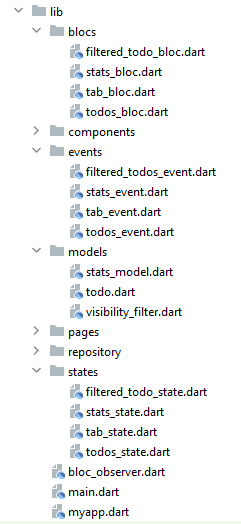
\includegraphics[width=0.4\textwidth]{Images/struttura_cartelle_bloc.png}
    \caption{Shows the final folders structure for the BLoC implementation of the Todos app}
    \label{fig:struttura_cartelle_bloc}
\end{figure}
Figure \ref{fig:widget_tree_structure_bloc}  represents the widget's tree structure for the BLoC final application. 

\begin{figure}[H]
    \centering
    \subfloat[Widgets tree structure \textit{todos }tab\label{fig:todos_tab_UI}]{
        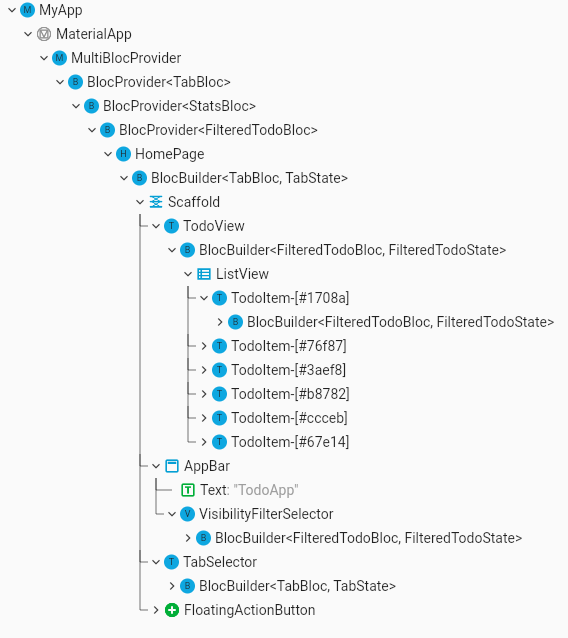
\includegraphics[scale=0.6]{Images/albero_bloc_todos.png}
    }
    \quad
    \subfloat[Widgets tree structure \textit{stats }tab\label{fig:todos_tab_tree}]{
        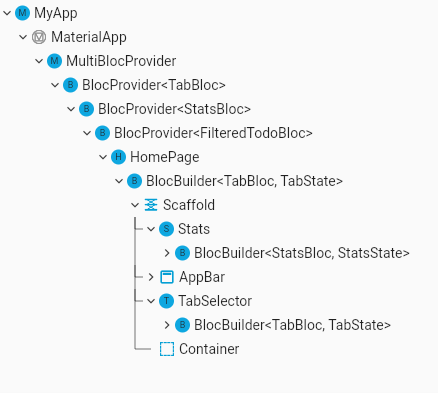
\includegraphics[scale=0.6]{Images/albero_bloc_stats.png}
    }
    \caption{Shows the widgets tree structure for BLoC Todos app}
    \label{fig:widget_tree_structure_bloc}
\end{figure}

